\subsection{Расчёт циклона}
\paragraph{Постановка задачи\\}
\addcontentsline{toc}{paragraph}{Постановка задачи}
В задаче рассматривается турбулентное течение вязкого газа с дисперсными включениями в циклоне модели Stairmand c учётом влияния дисперсной фазы на исходное течение. Геометрические параметры циклона представлены в \textit{таблице \ref{cycloneGeomPar}}.

  \begin{minipage}{0.6\textwidth}
    \captionof{table}{Геометрия фильтра}
    \label{cycloneGeomPar}
			\begin{tabular}{l l}
				\hline
				\label{geometrytable}
				Диаметр цилиндра, $D$ & $0.205m$ \\
				Диаметр выходной трубы, $D_e$ & $0.5D$ \\
				Высота входного канала, $a$ & $0.5D$ \\
				Ширина входного канала, $b$ & $0.2D$ \\
				Длина выходной трубы, $h_e$ & $0.75D$ \\
				Полная высота фильтра, $H$ & $4.0D$ \\
				Высота цилиндра, $h$ & $1.5D$ \\
				Диаметр нижнего сечения, $B$ & $0.36D$ \\
				Высота пылесборника, $h_d$ & $0.25D$ \\
				Диаметр пылесборника, $D_d$ & $0.75D$ \\
			\end{tabular}
    \end{minipage}
    \hspace{1em}
  \begin{minipage}{0.35\textwidth}
    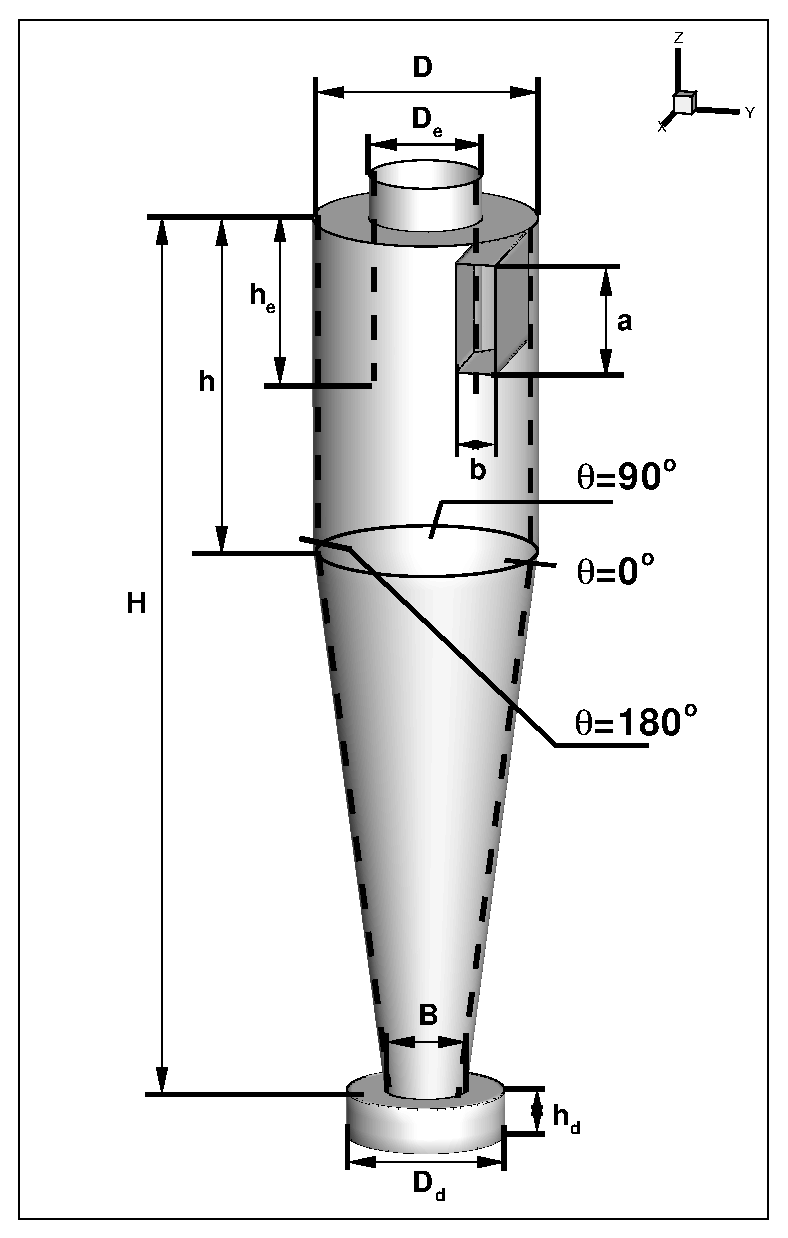
\includegraphics[scale=0.45]{cycloneGeometryTeta}
	\captionof{figure}{Схема фильтра}
	\label{fig:cycloneGeometryScheme}
  \end{minipage}
  \vspace{1em}
	
	Течение исследуется для 4 различных скоростей на входе, а также для трёх диаметров частиц. Граничные условия для задачи описаны в \textit{таблице \ref{cycloneBC}}, а на \textit{рисунке \ref{fig:cycloneMesh}} показана сетка расчётной области.
	
\begin{minipage}{0.6\textwidth}
    \captionof{table}{Граничные условия}
    \label{cycloneBC}
	\begin{tabular}{c}
		\hline
		\label{geometrytable}
		Скорость на входе, $U_{in}=$  $5, 10, 15, 20 m/s$ \\
		Температура на входе, $T_{in}=$  $300 K$ \\
		Температура частиц, ${T_p}_{in}=$  $300 K$ \\
		Скорость частиц на входе, ${U_p}_{in} = U_{in}$ \\
		Давление на выходе, $P_{out}=$  $1atm$ \\
		Тепловой поток на стенках, $q_w=$  $0$ \\
		Диаметр частиц, $d_p=$ $10^{-5}m, 10^{-6}m, 10^{-7}	m$\\
	\end{tabular}
\end{minipage}
\hspace{1em}
\begin{minipage}{0.35\textwidth}
    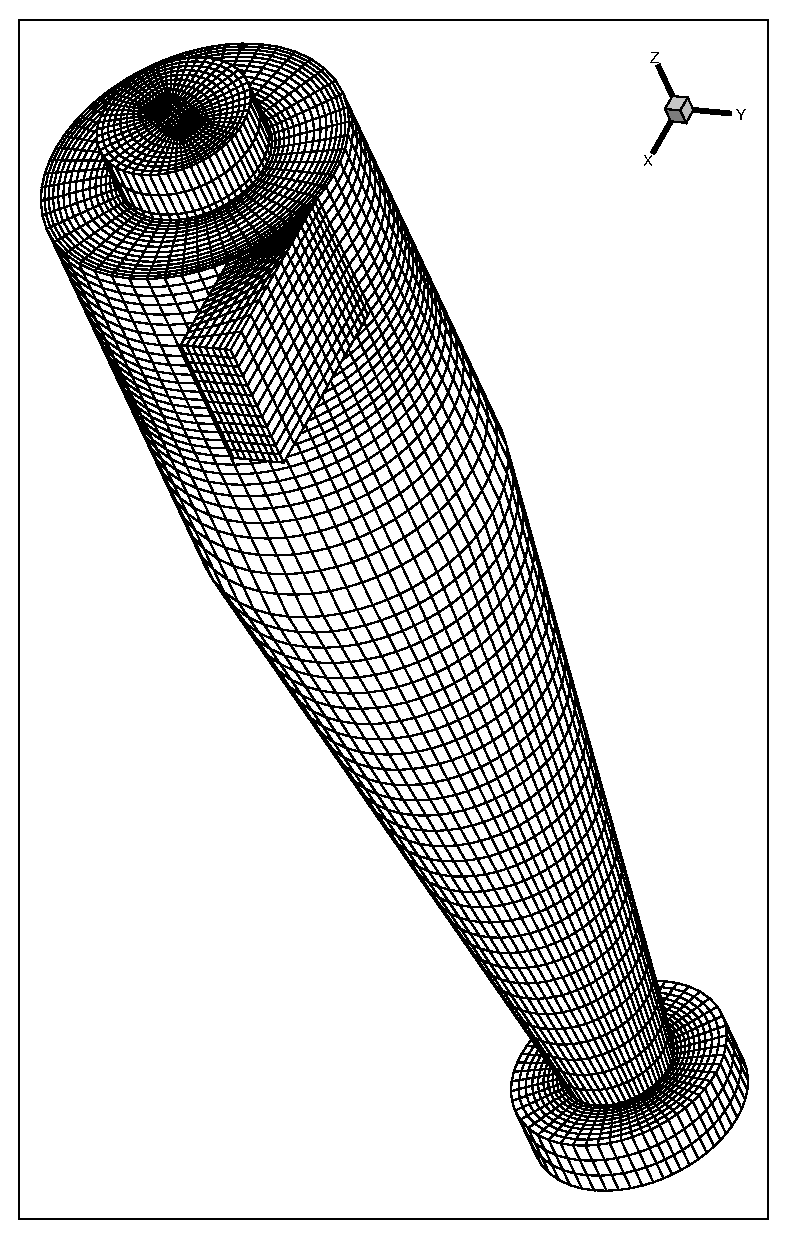
\includegraphics[scale=0.45]{meshCyclone}
	\captionof{figure}{Сетка расчётной области}
	\label{fig:cycloneMesh}
\end{minipage}
\vspace{1em}  
  \paragraph{Методические исследования\\}
  \addcontentsline{toc}{paragraph}{Методические исследования}

  Для исследования сеточной сходимости решения, расчёты задачи с  $U_{in} = 20m/s$ проводились на сетках 29380 ячеек, 96256 ячеек и 179552 ячейки. Сравнение профилей скорости вдоль двух отрезков, $1:$ $\left\{\left(0, 0, -0.3\right),\left(0.09, 0, -0,3\right)\right\}$ и $2:$ $\left\{\left(0, 0, -0.3\right),\left(0, 0.09, -0,3\right)\right\}$, представлены на \textit{рисунках \ref{fig:cycloneMeshIndependence1} -  \ref{fig:cycloneMeshIndependence4}}.
 \begin{figure}[h]
	\vspace{-1em}
	\begin{minipage}{0.475\linewidth}
		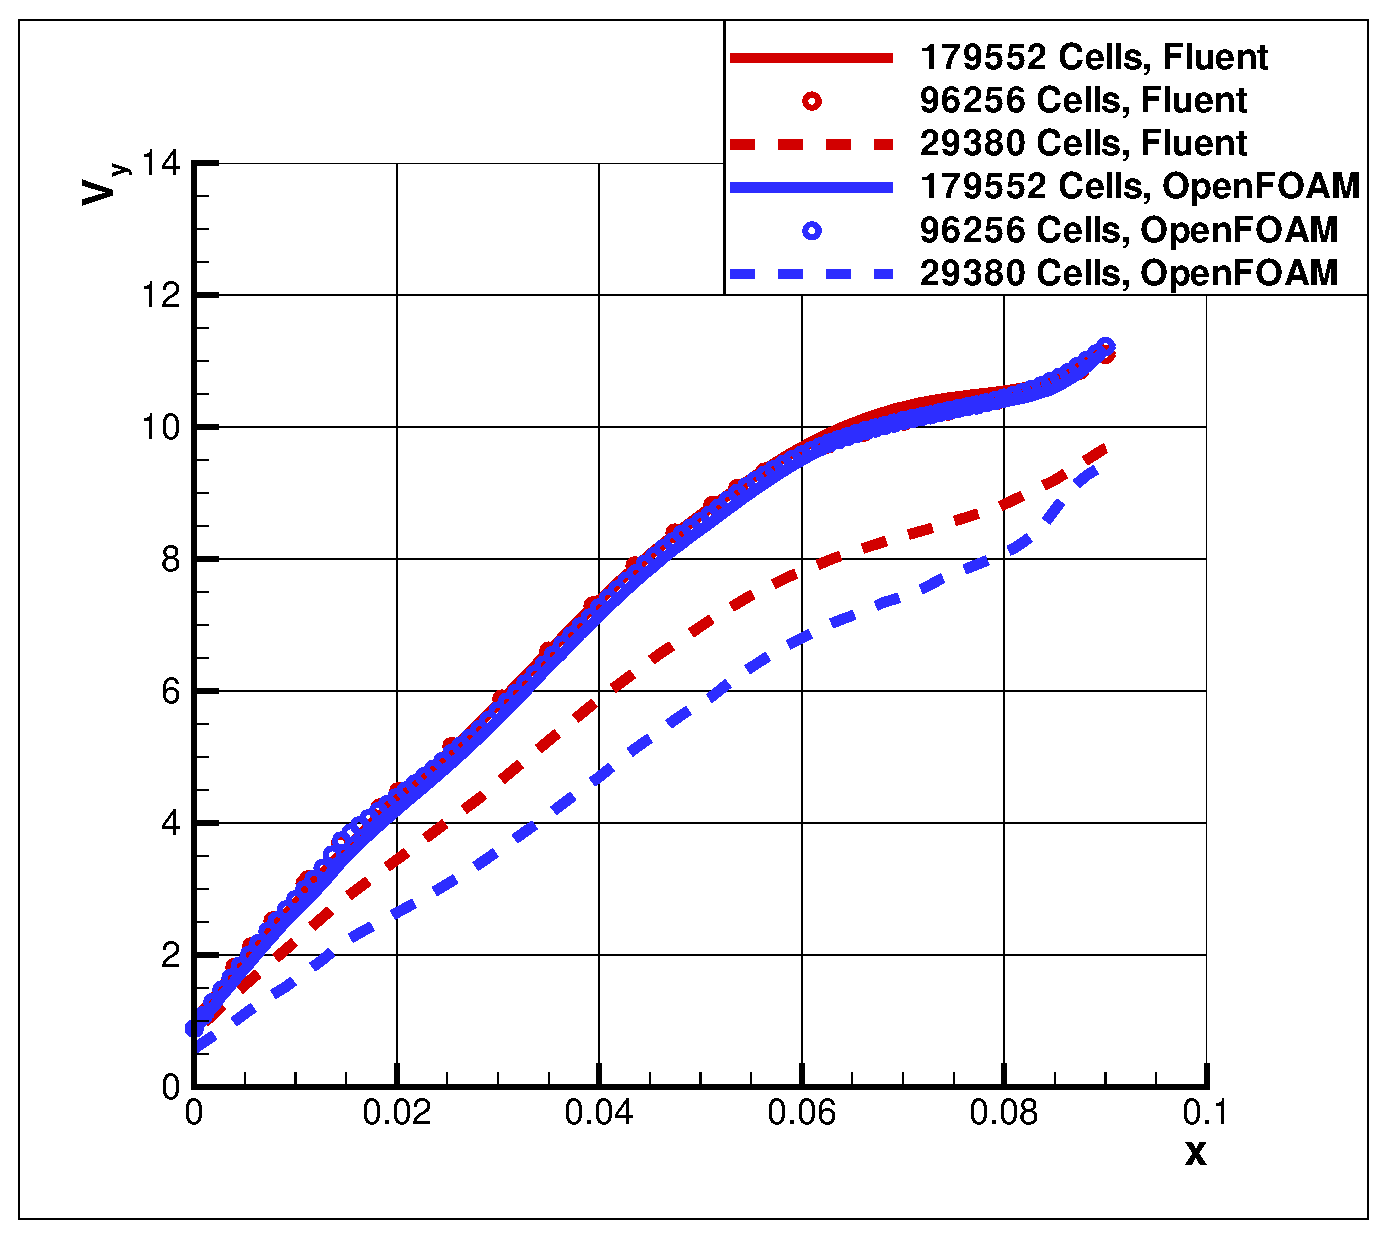
\includegraphics[scale=0.33]{cycloneMeshIndependence1}
		\caption{Профили $V_y$ вдоль прямой $1$}
		\label{fig:cycloneMeshIndependence1}
	\end{minipage}
	\hspace{0.5em}
	\begin{minipage}{0.475\linewidth}
		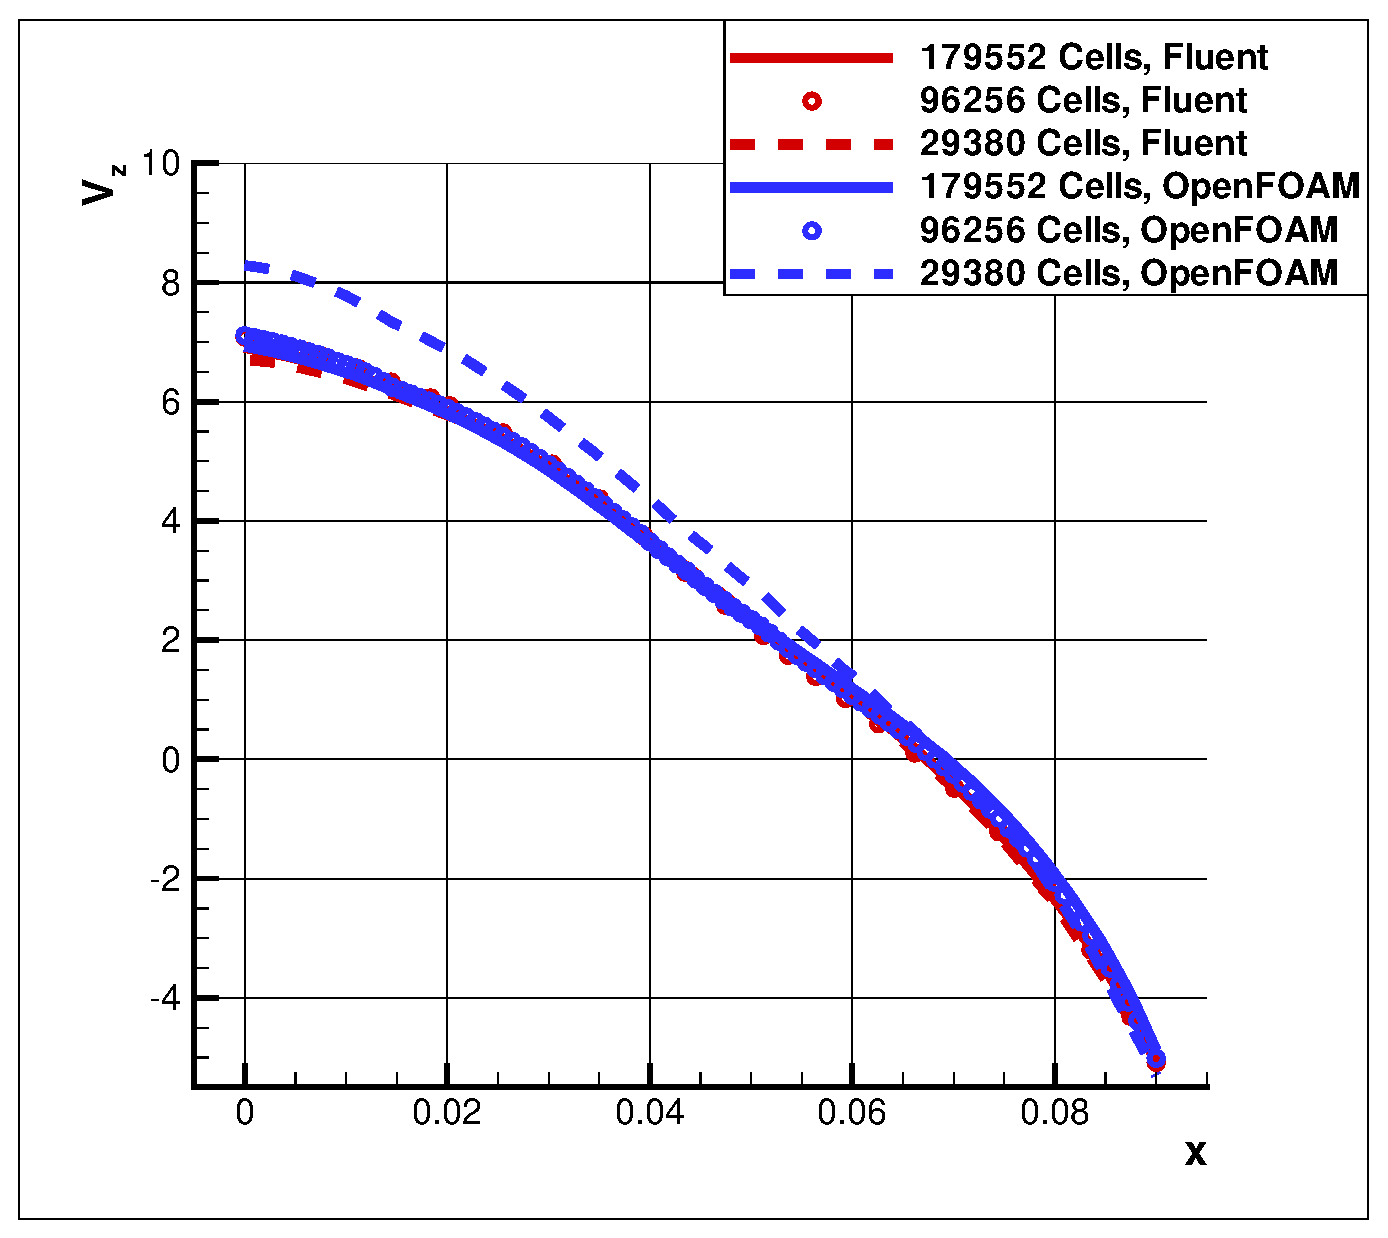
\includegraphics[scale=0.33]{cycloneMeshIndependence2}
		\caption{Профили $V_z$ вдоль прямой $1$}
		\label{fig:cycloneMeshIndependence2}
	\end{minipage}
\end{figure}

 \begin{figure}[h]
	\vspace{-1em}
	\begin{minipage}{0.475\linewidth}
		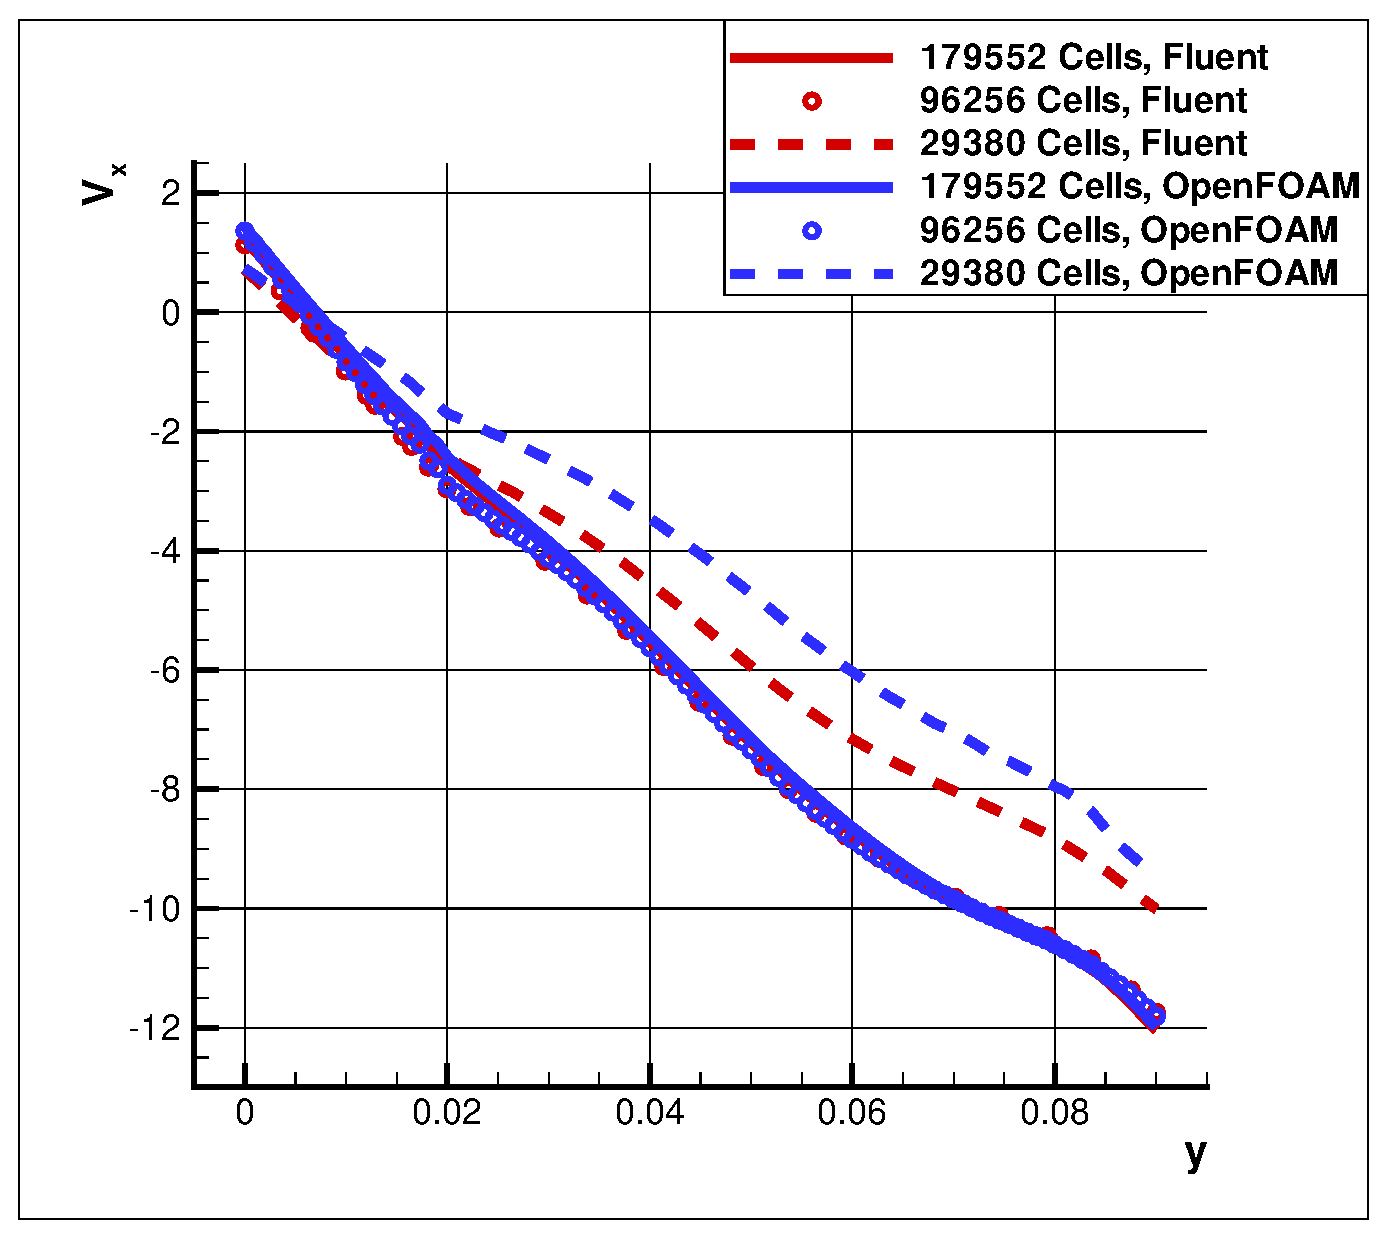
\includegraphics[scale=0.33]{cycloneMeshIndependence3}
		\caption{Профили $V_x$ вдоль прямой $2$}
		\label{fig:cycloneMeshIndependence3}
	\end{minipage}
	\hspace{0.5em}
	\begin{minipage}{0.475\linewidth}
		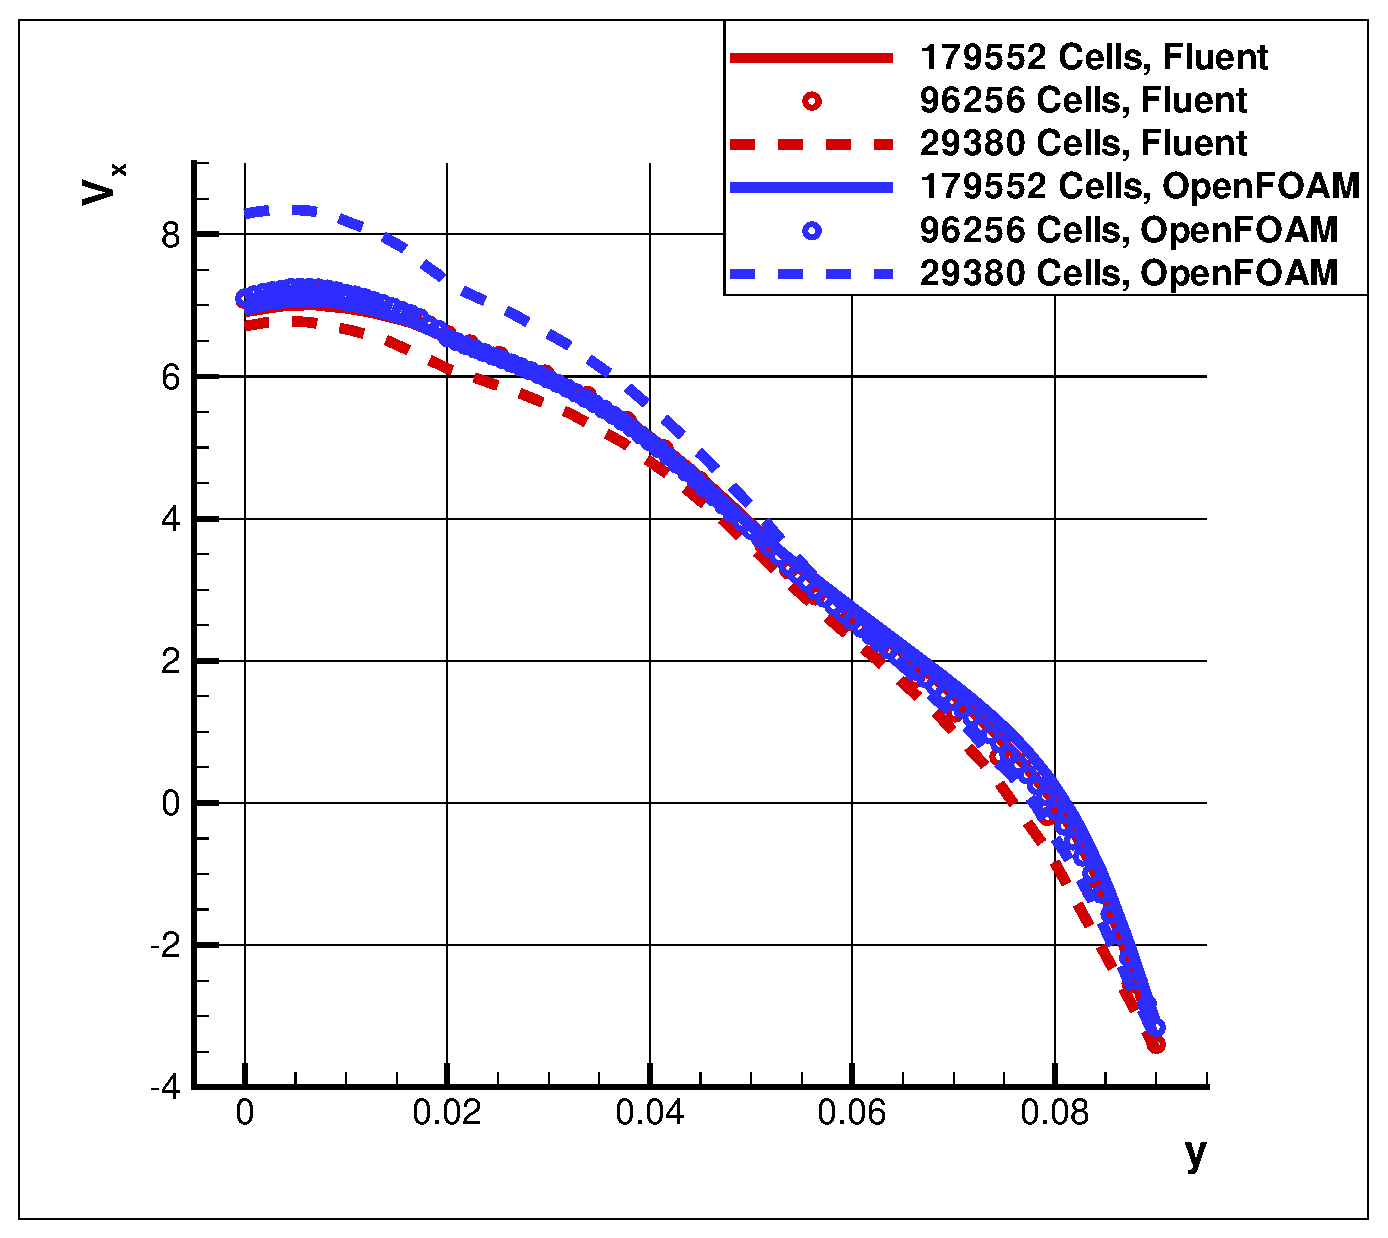
\includegraphics[scale=0.33]{cycloneMeshIndependence4}
		\caption{Профили $V_z$ вдоль прямой $2$}
		\label{fig:cycloneMeshIndependence4}
	\end{minipage}
\end{figure}
\clearpage
Видно, что решение на самой грубой сетке (29380 ячеек) сильно отличается от решения на более подробных сетках. В то же время, решение на сетках 96256 ячеек и 179552 ячейки отличаются менее, чем на 5\%, так что, сетки в 96256 ячеек вполне достаточно для получения сеточно-независимого решения. Кроме того, решения в Fluent и OpenFOAM прекрасно соответствуют друг другу -- профили скорости на \textit{рисунках \ref{fig:cycloneMeshIndependence1} -  \ref{fig:cycloneMeshIndependence4}} для Fluent и OpenFOAM практически неотличимы для подробных сеток.

\begin{figure}[h]
	\centering
	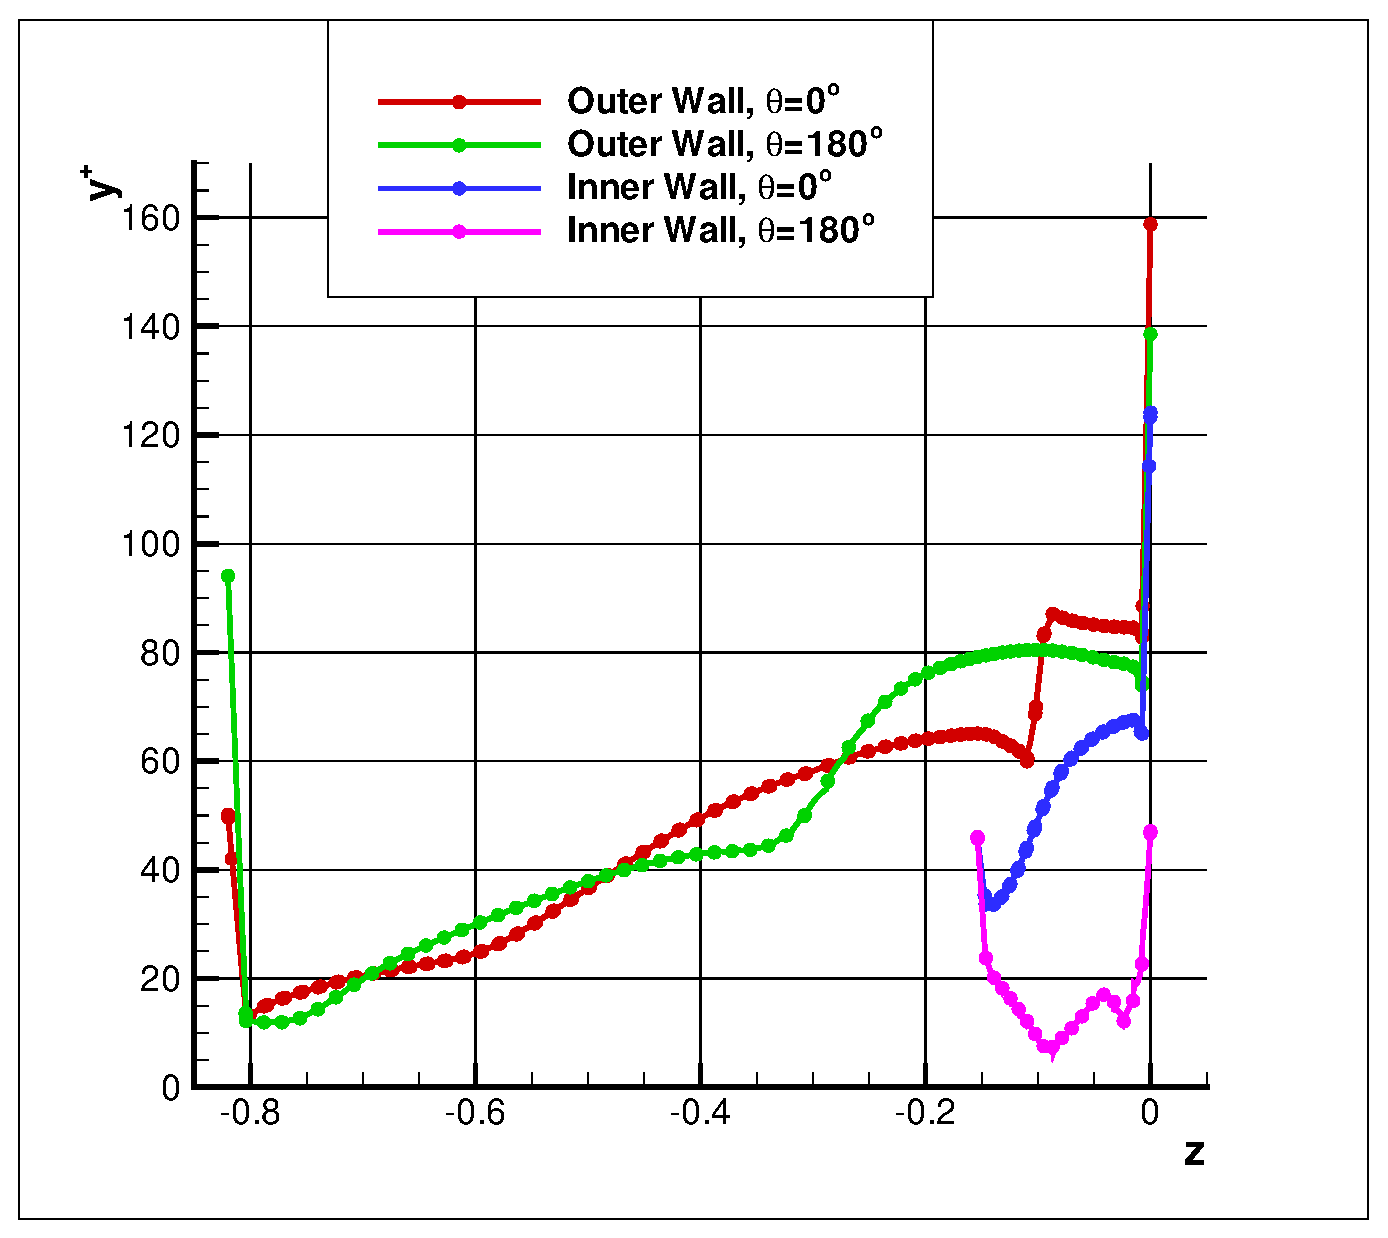
\includegraphics[scale=0.4]{yplusCyclone}
	\caption{Величина $y^{+}$ первой пристенной ячейки на внешней и внутренней стенках циклона}
	\label{fig:cycloneyPlus}
\end{figure}

На \textit{рисунке \ref{fig:cycloneyPlus}}, проиллюстрировано распределение величины $y^{+}$ первой пристенной ячейки, построенное вдоль образующих внешних и внутренных стенок, для углов $\theta=0^o$ и $\theta=180^o$ (отмечены на \textit{рисунке \ref{fig:cycloneGeometryScheme}} пунктирными линиями). Из графиков видно, что в большей части области величина $y^{+}$ лежит в пределах $10 \div 90$, что вполне адекватно для использования модели Ментера с автоматическими пристеночными функциями.
